%
\section{Evaluation}
\label{sect:evaluation} %

In this section, we discuss an evaluation of \agl. Our aim is to show that \agl~is both  essentially expressive and practically usable.
%
In this paper, we focus on evaluating \agl~because it is a new language contribution of our method. We consider \agl~as a type of specification language and adapt the \dcsl~evaluation approach that we applied in~\cite{le_domain_2018}.
%
More specifically, we adapt from~\cite{lamsweerde_formal_2000} the following three criteria for evaluating \agl: expressiveness, required coding level, and constructibility. We will present our evaluation of these criteria in Sections~\ref{sect:eval-expressiveness}--\ref{sect:eval-construct}. We conclude in Section~\ref{sect:eval-discussion} with a number of discussion points concerning the evaluation.
%
\subsection{Expressiveness} \label{sect:eval-expressiveness}
This is the extent to which a language is able to express the properties of interest of its domain~\cite{lamsweerde_formal_2000}. For \agl, the domain properties are captured as meta-concepts and associations in the language's ASM. We measure the expressiveness of \agl~by showing how it is able to express the five essential UML activity modeling patterns that we presented in~\cite{le_domain_2018}. We named the patterns after these five elementary activity flows: sequential, decisional, forked, joined and merged. Combinations of the patterns are used to build complete software. In this paper, we extend each pattern solution (presented in~\cite{le_domain_2018}) with an AGC in order to express the configured unified model.

We are particularly interested in the design of the \textit{pattern form}~\cite{riehle_understanding_1996, gamma_design_1994}. To keep the patterns generic, we present for each pattern form a UML activity model and a \textbf{template configured unified model} that realises it. The template model is a `parameterised' configured unified model, in which elements of the nonannotation meta-concepts are named after the generic roles that they play. 
%
For brevity, we will omit all associative fields and base domain methods from the model's diagram.

Similar to~\cite{le_domain_2018}, we illustrate each pattern with a variant of the unified model for the enrolment management activity of \courseman. A pattern example includes a configured unified model and one or more software GUIs. In this paper, we will focus on presenting the configured unified model and, in particular, its AGC. Please refer to~\cite{le_domain_2018, le_domain_2017} for details about the unified model and the software GUI of each example. 
The \courseman~software of each example is automatically generated from the configured unified model, using the software tool described in Section~\ref{sect:tool}. 
%Please refer to our tool's manual for how to run it with this case study.
%
\subsubsection{Sequential Pattern Form} \label{sect:eval-expressiveness-sequential}
%
\begin{figure*}[ht]
\begin{center}
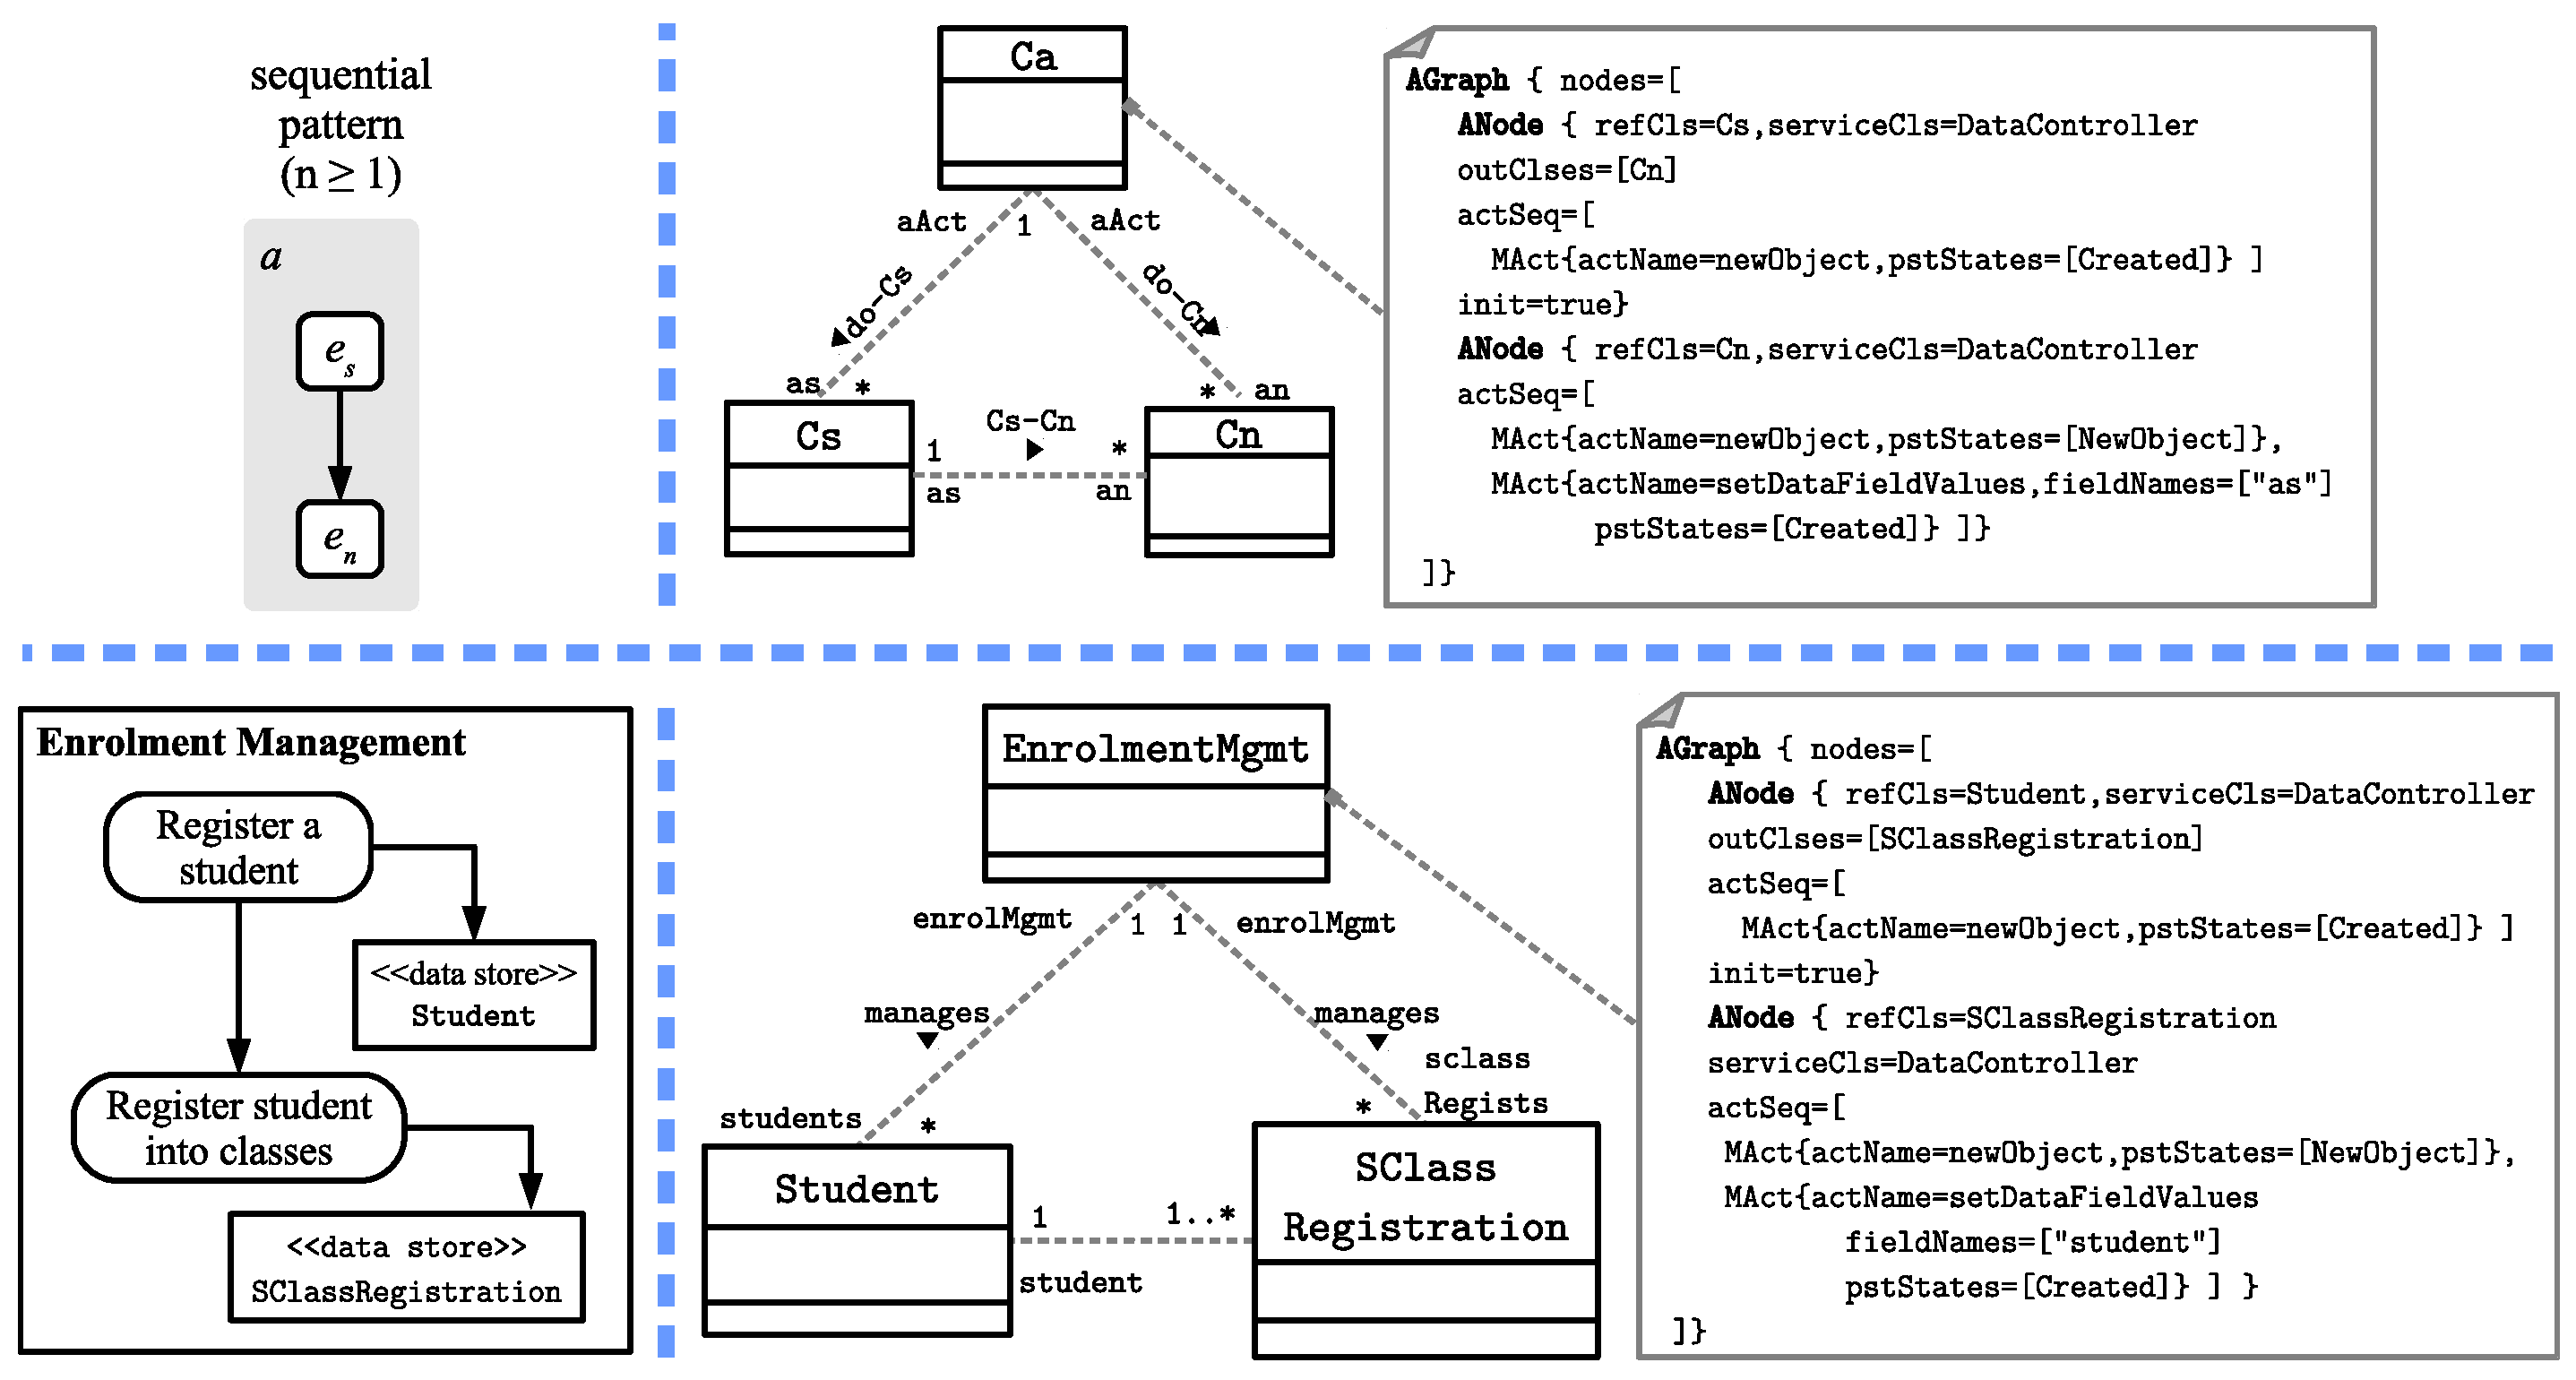
\includegraphics[scale=0.33]{case-study/sequential-form}
\end{center}
\caption{The sequential pattern form.} %
\label{fig:sequential-form}
\end{figure*}
%
\begin{figure*}[ht]
\begin{center}
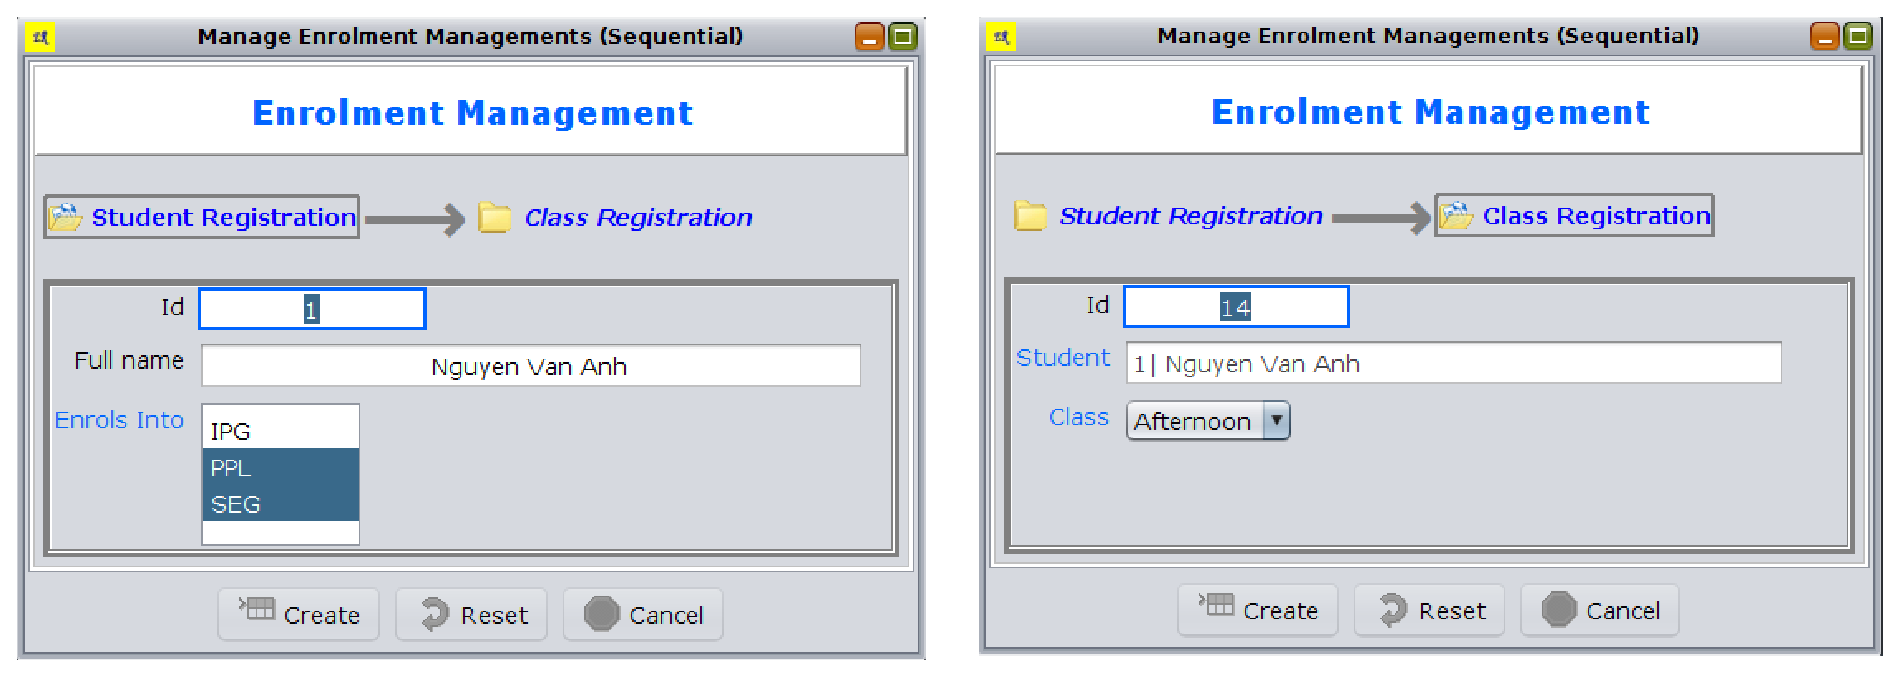
\includegraphics[scale=0.5]{case-study/sequential-form-eg-gui}
\end{center}
\caption{The sequential pattern form view of enrolment management activity.} %
\label{fig:sequential-form-eg-gui}
\end{figure*}

The top-left of Figure~\ref{fig:sequential-form} shows the UML activity model, while the top-right shows the template configured unified model.
This model consists of three classes \clazz{Ca}, \clazz{Cs}, and \clazz{Cn}. Class \clazz{Ca} is the activity class and has two associations with the two data classes \clazz{Cs} and \clazz{Cn}. These are the \textit{ref} domain classes of the two action nodes $ e_s $ and $ e_n $, \resp

The AGC is given in the \clazz{AGraph}'s note box in the top-right corner of the figure. It consists of two \clazz{ANode}s. The first \clazz{ANode} specifies node $ e_s $, and the second specifies node $ e_n $. The \clazz{ANode}s are quite self-explanatory except for the three \clazz{MAct}s, which are worth some explanation. The first \clazz{MAct}'s configuration specifies the SAA \amos{newObject}{Created}). This SAA is a subset of the one presented in Section~\ref{sect:arch-saa}. It involves performing \atomact{newObject}{ NewObject} and any combination of \atomact{setDataFieldValues}{Editing} and \atomact{createObject}{Created}. Action \membern{newObject} is to prepare \clazz{Cs}' view for user to enter input. Action \membern{setDataFieldValues} is to set a view field's value from each user input (allowing user to re-enter if an error occurs). And action \membern{createObject} is to create a new \clazz{Cs}' object from the input.

The second and third \clazz{MAct}s together perform a similar logic over \clazz{Cn}, except for the need to break the \membern{setDataFieldValues} operation into two steps: \textit{(a)} set the \clazz{Cs} object created by the first \clazz{MAct} (and offered by $ e_s $ to $ e_n $ via its output pin) into a suitable view field of \clazz{Cn}'s view and (\textit{b)} set values of other view fields (allowing user to re-enter if an error occurs). To achieve this, the second \clazz{MAct} first specifies \amos{newObject}{NewObject}. The third \clazz{MAct} then specifies the rest of the logic. Step \textit{(a)} is performed by the operation \membern{setDataFieldValues}, which uses the field named \strq{as} to identify the view field of \clazz{Cn}'s view whose value needs to be set. Step \textit{(b)} is performed by \membern{setDataFieldValues} (as explained above) for other view fields.
%
\subsubsection*{Example}
The bottom of Figure~\ref{fig:sequential-form} shows how the pattern is applied to a simple variant of the \courseman's enrolment management activity. The UML activity model involves performing two actions in sequence. The first action (\clazz{Student}) registers a student into course modules, while the second action (\clazz{SClassRegistration}) registers the student into a preferred class.

In this example: \clazz{Ca} = \clazz{EnrolmentMgmt}, \clazz{Cs} = \clazz{Student}, $ n $ = 1, \clazz{C1} = \clazz{SClassRegistration}.

The two GUI snapshots of the example are shown in Figure~\ref{fig:sequential-form-eg-gui}: one snapshot for the view of the one action. Each view is embedded in the \clazz{EnrolmentMgmt}'s view. The overall layout is a tab layout and the view of each associated module is contained in a tab of this layout. The left-hand-side figure shows the tab containing the \clazz{Student}'s view, while the right-hand-side one shows the tab containing the \clazz{SClassRegistration}'s view. Note, in particular, that the view field of the field \clazz{SClassRegistration}.\attribn{student} (field \attrib{Cn}{as} in the template model) is automatically set to the \objc{Student}{\attribn{name}=\strq{Nguyen~Van~Anh}}, which is created on the \clazz{Student}'s view.
%
\subsubsection{Decisional Pattern Form} \label{sect:eval-expressiveness-decisional}
%
\begin{figure*}[ht]
\begin{center}
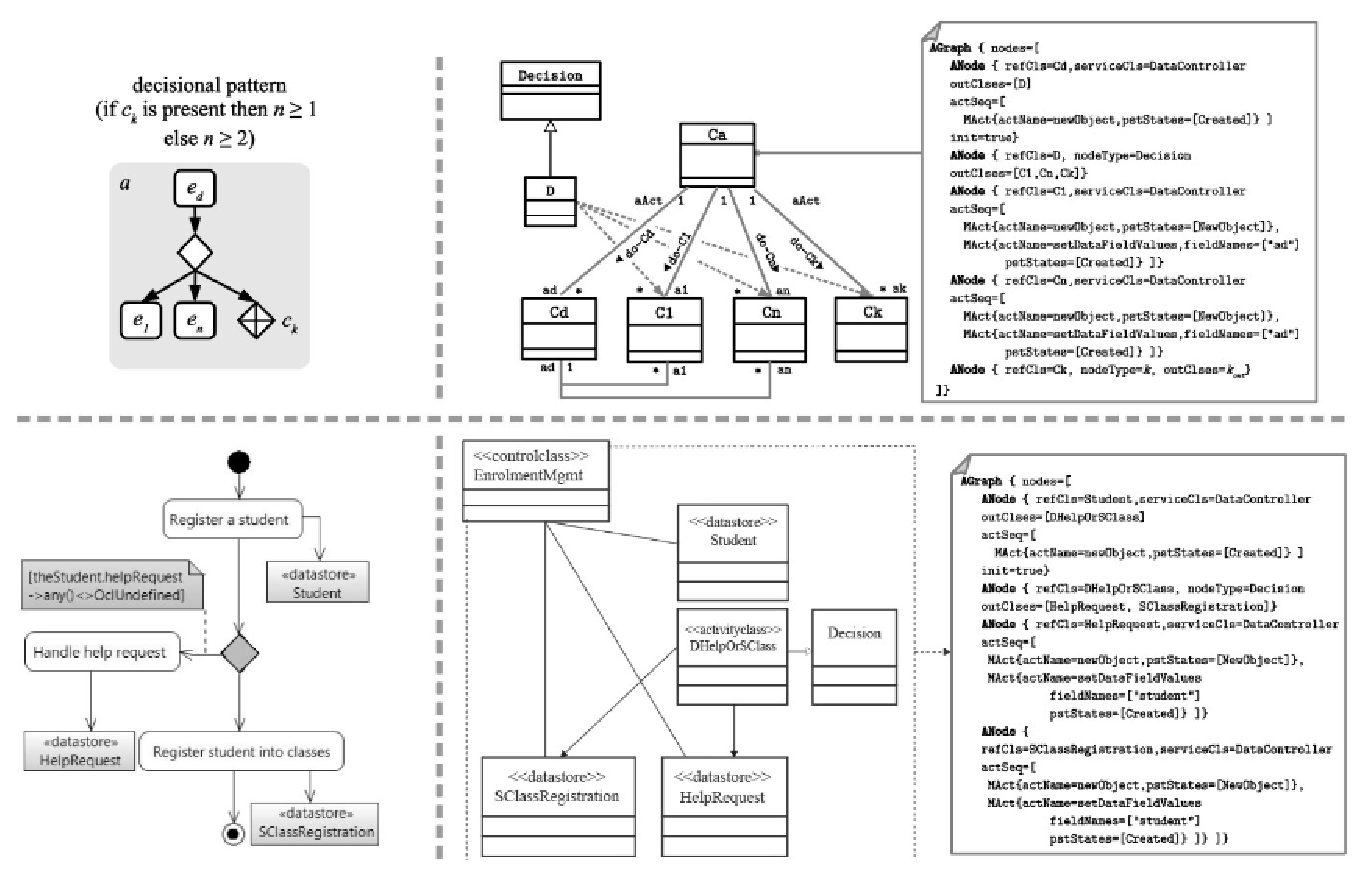
\includegraphics[scale=0.25
  ]{case-study/decisional-form}
\end{center}
\caption{The decisional pattern form.} %
\label{fig:decisional-form}
\end{figure*}
%
\begin{figure*}[ht]
\begin{center}
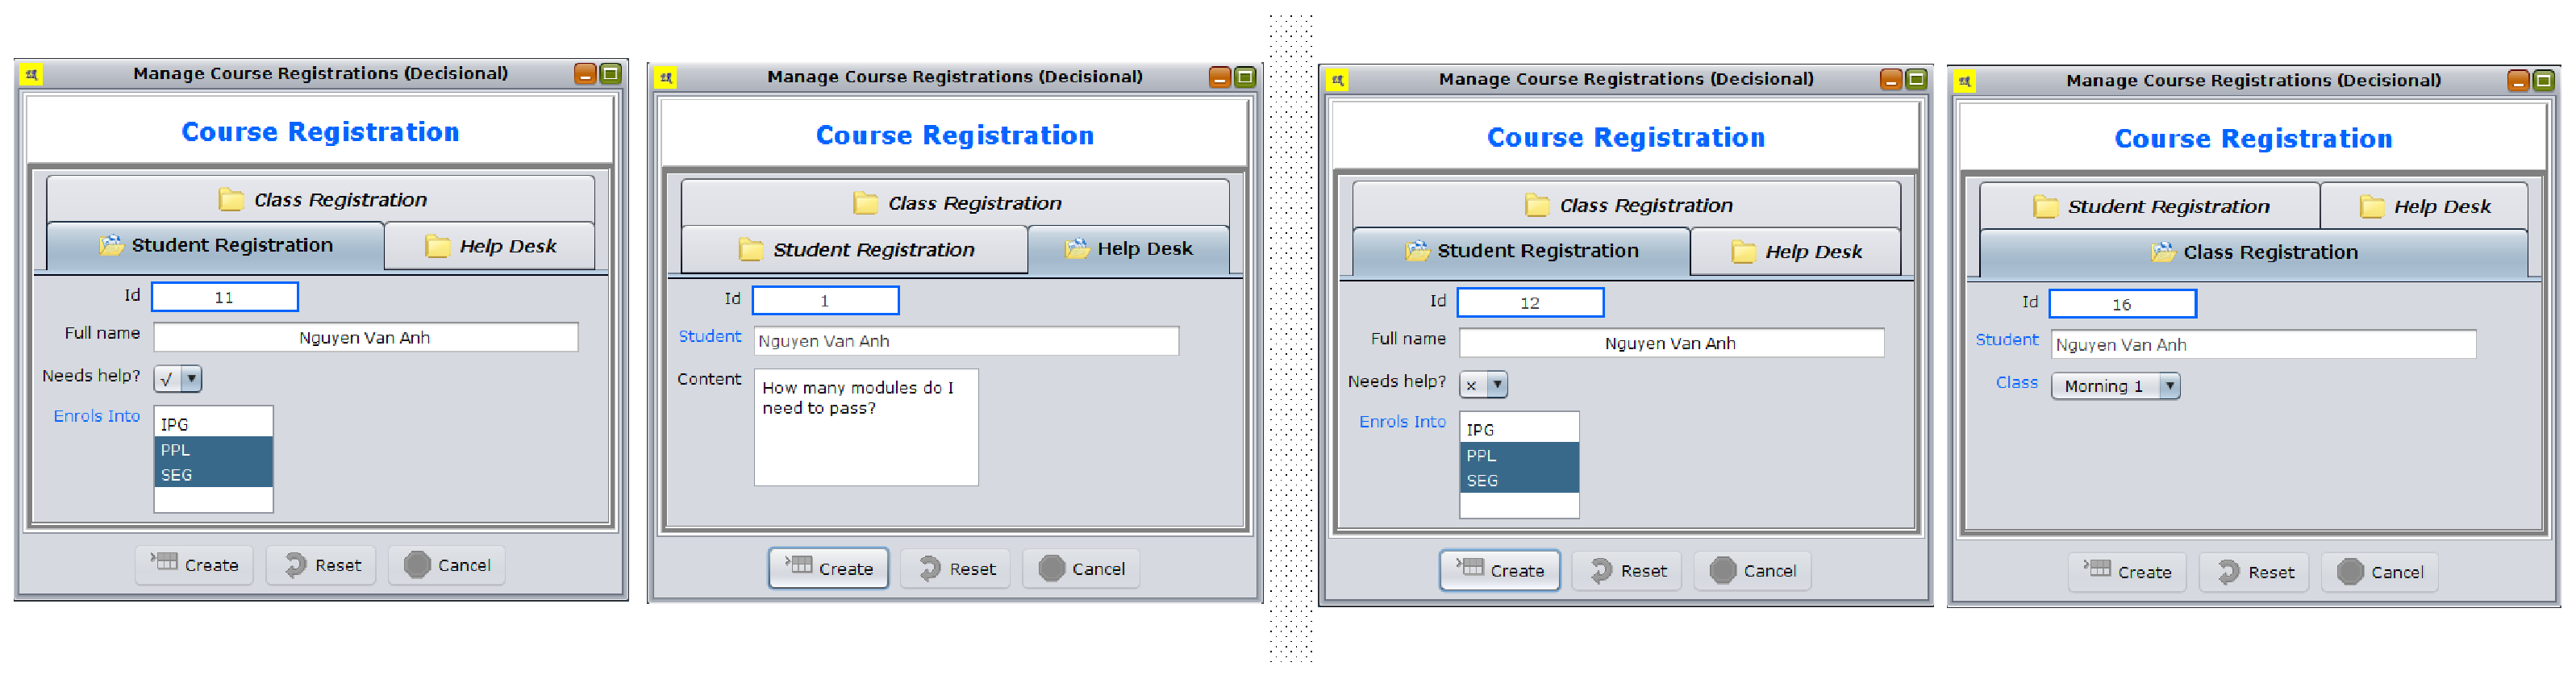
\includegraphics[scale=0.42
  ]{case-study/decisional-form-eg-gui}
\end{center}
\caption{The decisional pattern form view of enrolment management.} %
\label{fig:decisional-form-eg-gui}
\end{figure*}

The top-left of Figure~\ref{fig:decisional-form} shows the UML activity model, while the top-right shows the template configured unified model. Apart from the activity class \clazz{Ca}, this model includes five other domain classes, namely \clazz{Cd}, \clazz{D}, \clazz{C1}, \clazz{Cn}, and \clazz{Ck}, that are mapped to the five activity nodes. In particular, class \clazz{Ck} is a control class that is referenced by the control node $c_k$ of the activity model. 
Class \clazz{D} is a decision class, which implements the \clazz{Decision} interface.
%
Since the decision's logic may require knowledge of the domain classes involved (namely \clazz{C1}, \clazz{Cn}, and \clazz{Ck}), there are (optional) weak dependency associations between \clazz{D} and these classes. Depending on the domain requirements, we would need none or some of these associations.

Class \clazz{Ca} has one-many associations to the other four domain classes. 
Note that the association to \clazz{Ck} can be used as a bridge in a larger activity model to other activity flow blocks. This association is applied differently if $ c_k $ is a decision node. In this case, \clazz{Ck} has no associations and thus the association to \clazz{Ck} is replaced by (or ``unfolded'' into) a set of associations that connect \clazz{Ca} directly to the domain classes of the model containing \clazz{Ck}.

In the template model, the two associations between \clazz{Cd} and \clazz{C1}, \clazz{Cn} reflect the fact that both \clazz{C1} and \clazz{Cn} know about \clazz{Cd}, due to the passing of object tokens from $ e_d $ to $ e_1 $ and $ e_n $ (via the decision node).

The AGC consists of five \clazz{ANode}s. The first \clazz{ANode} is to create a new \clazz{Cd} object. The second \clazz{ANode} is to run the decision logic. The third and fourth \clazz{ANode}s represent the two decision cases: the first results in creating a new \clazz{C1} object for the specified \clazz{Cd} object, the second, which is repeated for all $ n $, results in creating a new \clazz{Cn} object for the same \clazz{Cd}. The fifth \clazz{ANode} is used for the case that \clazz{Ck} is specified. It uses two variables $ k $ and $ k_{out} $, both are dependent on \clazz{Ck}. Variable $ k $ specifies the control node type, while variable $ k_{out} $ specifies the array of output domain classes of \clazz{Ck}.

\subsubsection*{Example}
The bottom of Figure~\ref{fig:decisional-form} shows how the pattern is applied to the variant of \courseman's enrolment management activity that we introduced in the example of Section~\ref{sect:unified-domain-modeling}. The configured unified model, however, is a more detailed version of the one presented in Figures~\ref{fig:unified-model-example} and~\ref{fig:agc-enrolmentmgmt}. 

In this example: \clazz{Ca} = \clazz{EnrolmentMgmt}, \clazz{Cd} = \clazz{Student}, \clazz{D} = \clazz{DHelpOrSClass}, $ n $ = 2, \clazz{C1} = \clazz{HelpRequest}, \clazz{C2} = \clazz{SClassRegistration}.
The control node $ c_k $ is not specified.

The three GUI snapshots of the example are shown in Figure~\ref{fig:decisional-form-eg-gui}. The first GUI is for student registration. The second and third GUIs are for the cases that help request is and is not requested (\resp). Similar to the GUI of the sequential pattern, the activity's GUI contains the GUIs of the three actions in separate tabs. Under both cases of the decision, the \clazz{Student} object that is created in the first action (\eg \clazz{Student}(\attribn{name}=``Nguyen Van Anh'')) is passed on to the next action. This object is then presented in the data field of the associative field \attribn{student} of the domain class referenced by this action.
%
\subsubsection{Forked Pattern Form} \label{sect:eval-expressiveness-forked}
%
\begin{figure*}[ht]
\begin{center}
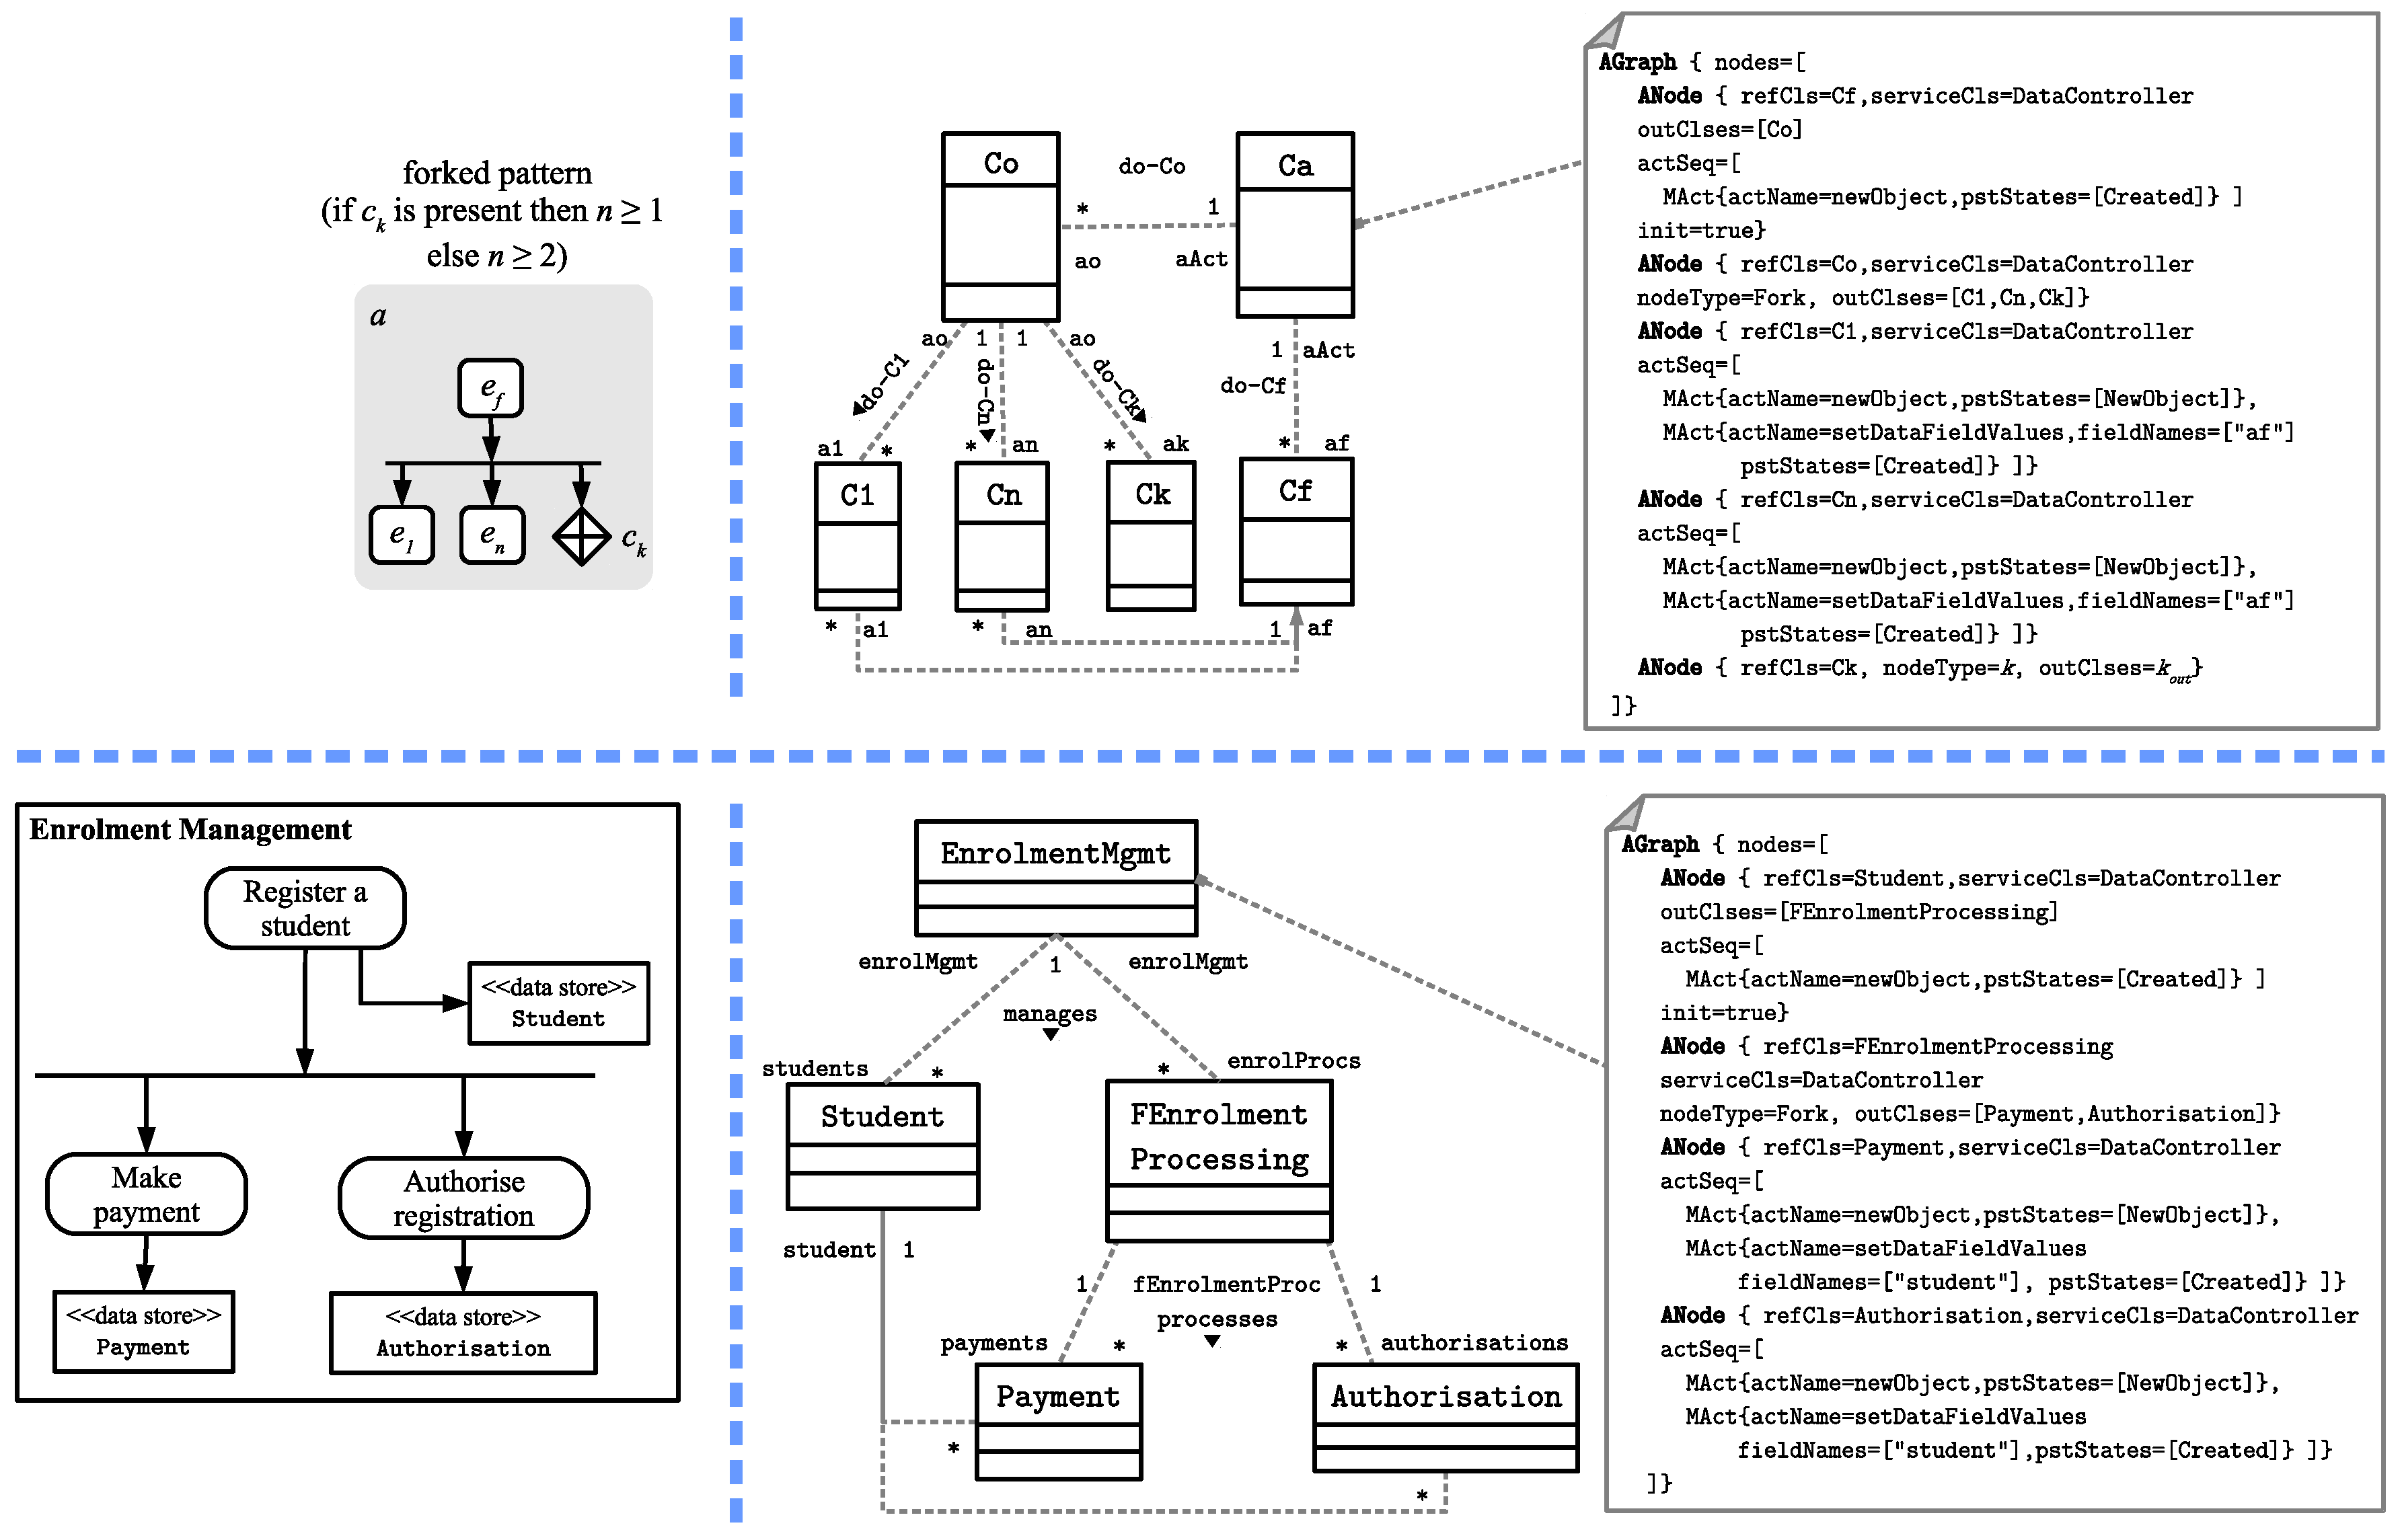
\includegraphics[scale=0.28 % 0.3
  ]{case-study/forked-form}
\end{center}
\caption{The forked pattern form.} %
\label{fig:forked-form}
\end{figure*}
%
\begin{figure*}[ht]
\begin{center}
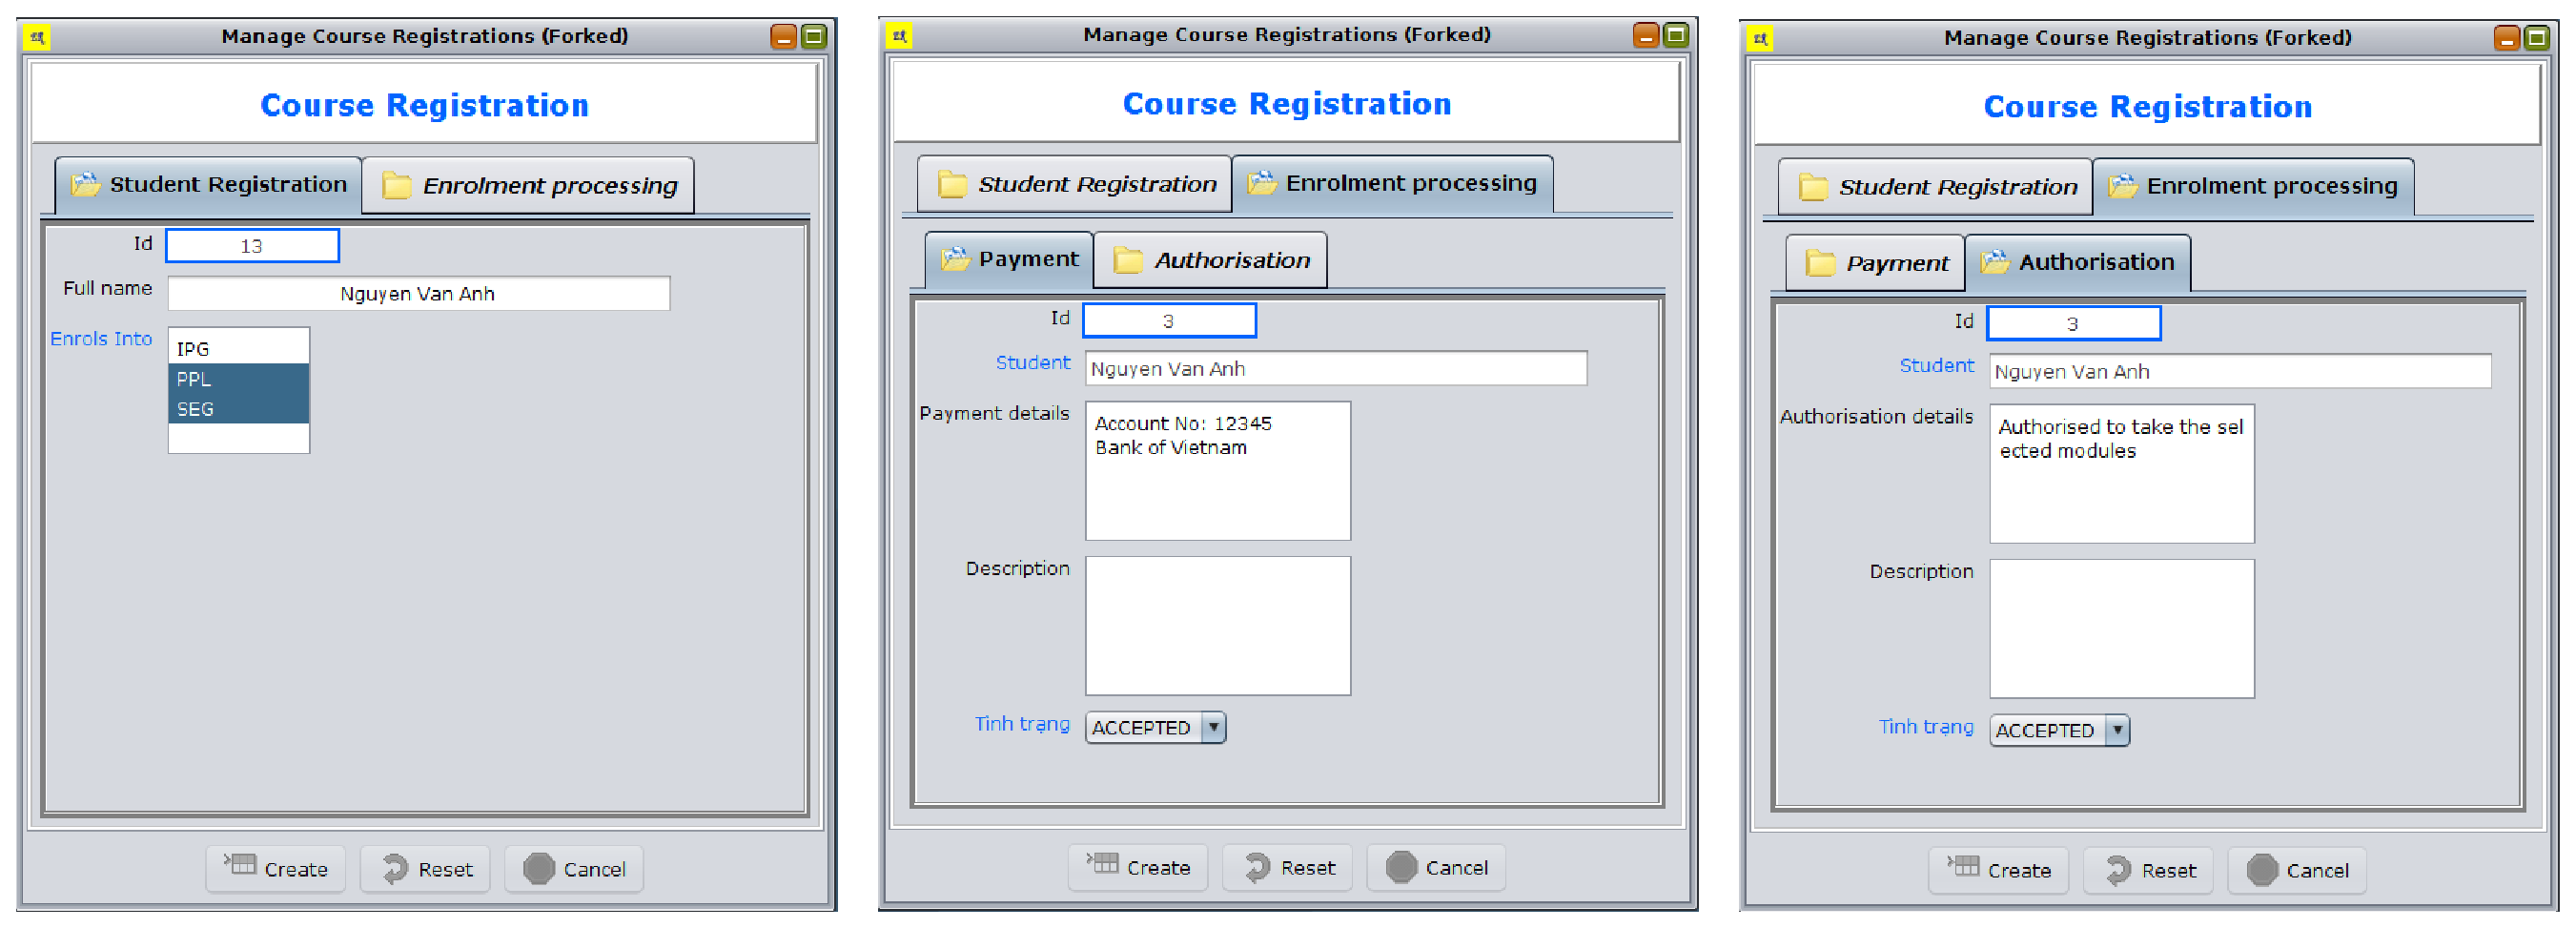
\includegraphics[scale=0.37 %0.4
  ]{case-study/forked-form-eg-gui}
\end{center}
\caption{The forked pattern form view of enrolment management activity.} %
\label{fig:forked-form-eg-gui}
\end{figure*}

The top-left of Figure~\ref{fig:forked-form} shows the UML activity model, while the top-right shows the template configured unified model. The activity class \clazz{Ca} has two associations to domain class \clazz{Cf} (referenced by node $ e_f $) and control class \clazz{Co} (referenced by the forked node). Class \clazz{Co} in turn has associations to the other three domain classes, namely \clazz{C1}, \clazz{Cn}, and \clazz{Ck}. In addition to these, class \clazz{Cf} has two associations to \clazz{C1} and \clazz{Cn}, as these classes need to know \clazz{Cf} through object passing.

Similar to the decisional activity's template model, we consider the case that the class \clazz{Ck} is not a decision class. When this class is a decision class, we unfold it into the template model.

The AGC is very similar to that of the decisional activity's template model, except for in the second \clazz{ANode}: the reference class is \clazz{Co} (as opposed to \clazz{D}), the node type is \code{Fork} and property \attribn{serviceCls} is \clazz{DataController}. This property configuration makes explicit the fact that \clazz{Co}'s module service is available for use if needed.
%
\subsubsection*{Example}
The bottom of Figure~\ref{fig:forked-form} shows how the pattern is applied to another variant of the \courseman's enrolment management. The UML activity model of this variant involves performing student registration ($ e_f $) and then two support actions concurrently: payment processing ($ e_1 $) and enrolment authorisation ($ e_2 $). These actions must be completed in order for any subsequent actions to proceed.

In this example: \clazz{Ca} = \clazz{EnrolmentMgmt}, \clazz{Cf} = \clazz{Student}, \clazz{Co} = \clazz{FEnrolmentProcessing}, $ n = 2 $, \clazz{C1} = \clazz{Payment}, \clazz{C2} = \clazz{Auhorisation}.

The three GUI snapshots of the example are shown in Figure~\ref{fig:forked-form-eg-gui}: one snapshot for one action. The first snapshot is for the first action (student registration). The second and third snapshots are for the two concurrent actions (\resp): making payment and enrolment authorisation. A difference between this GUI and the GUIs of the previous two patterns is that it has a 2-level containment. This 2-level containment reflects the length-2 association chain from \clazz{EnrolmentMgmt} (the activity class) to \clazz{Payment} and \clazz{Authorisation}. The first-level containment is that between the activity's GUI and \clazz{Student}'s and enrolment processing's GUI. The second-level containment is that between enrolment processing's GUI and \clazz{Payment}'s and \clazz{Authorisation}'s GUI.

%
\subsubsection{Joined Pattern Form} \label{sect:eval-expressiveness-joined}
%
\begin{figure*}[ht]
\begin{center}
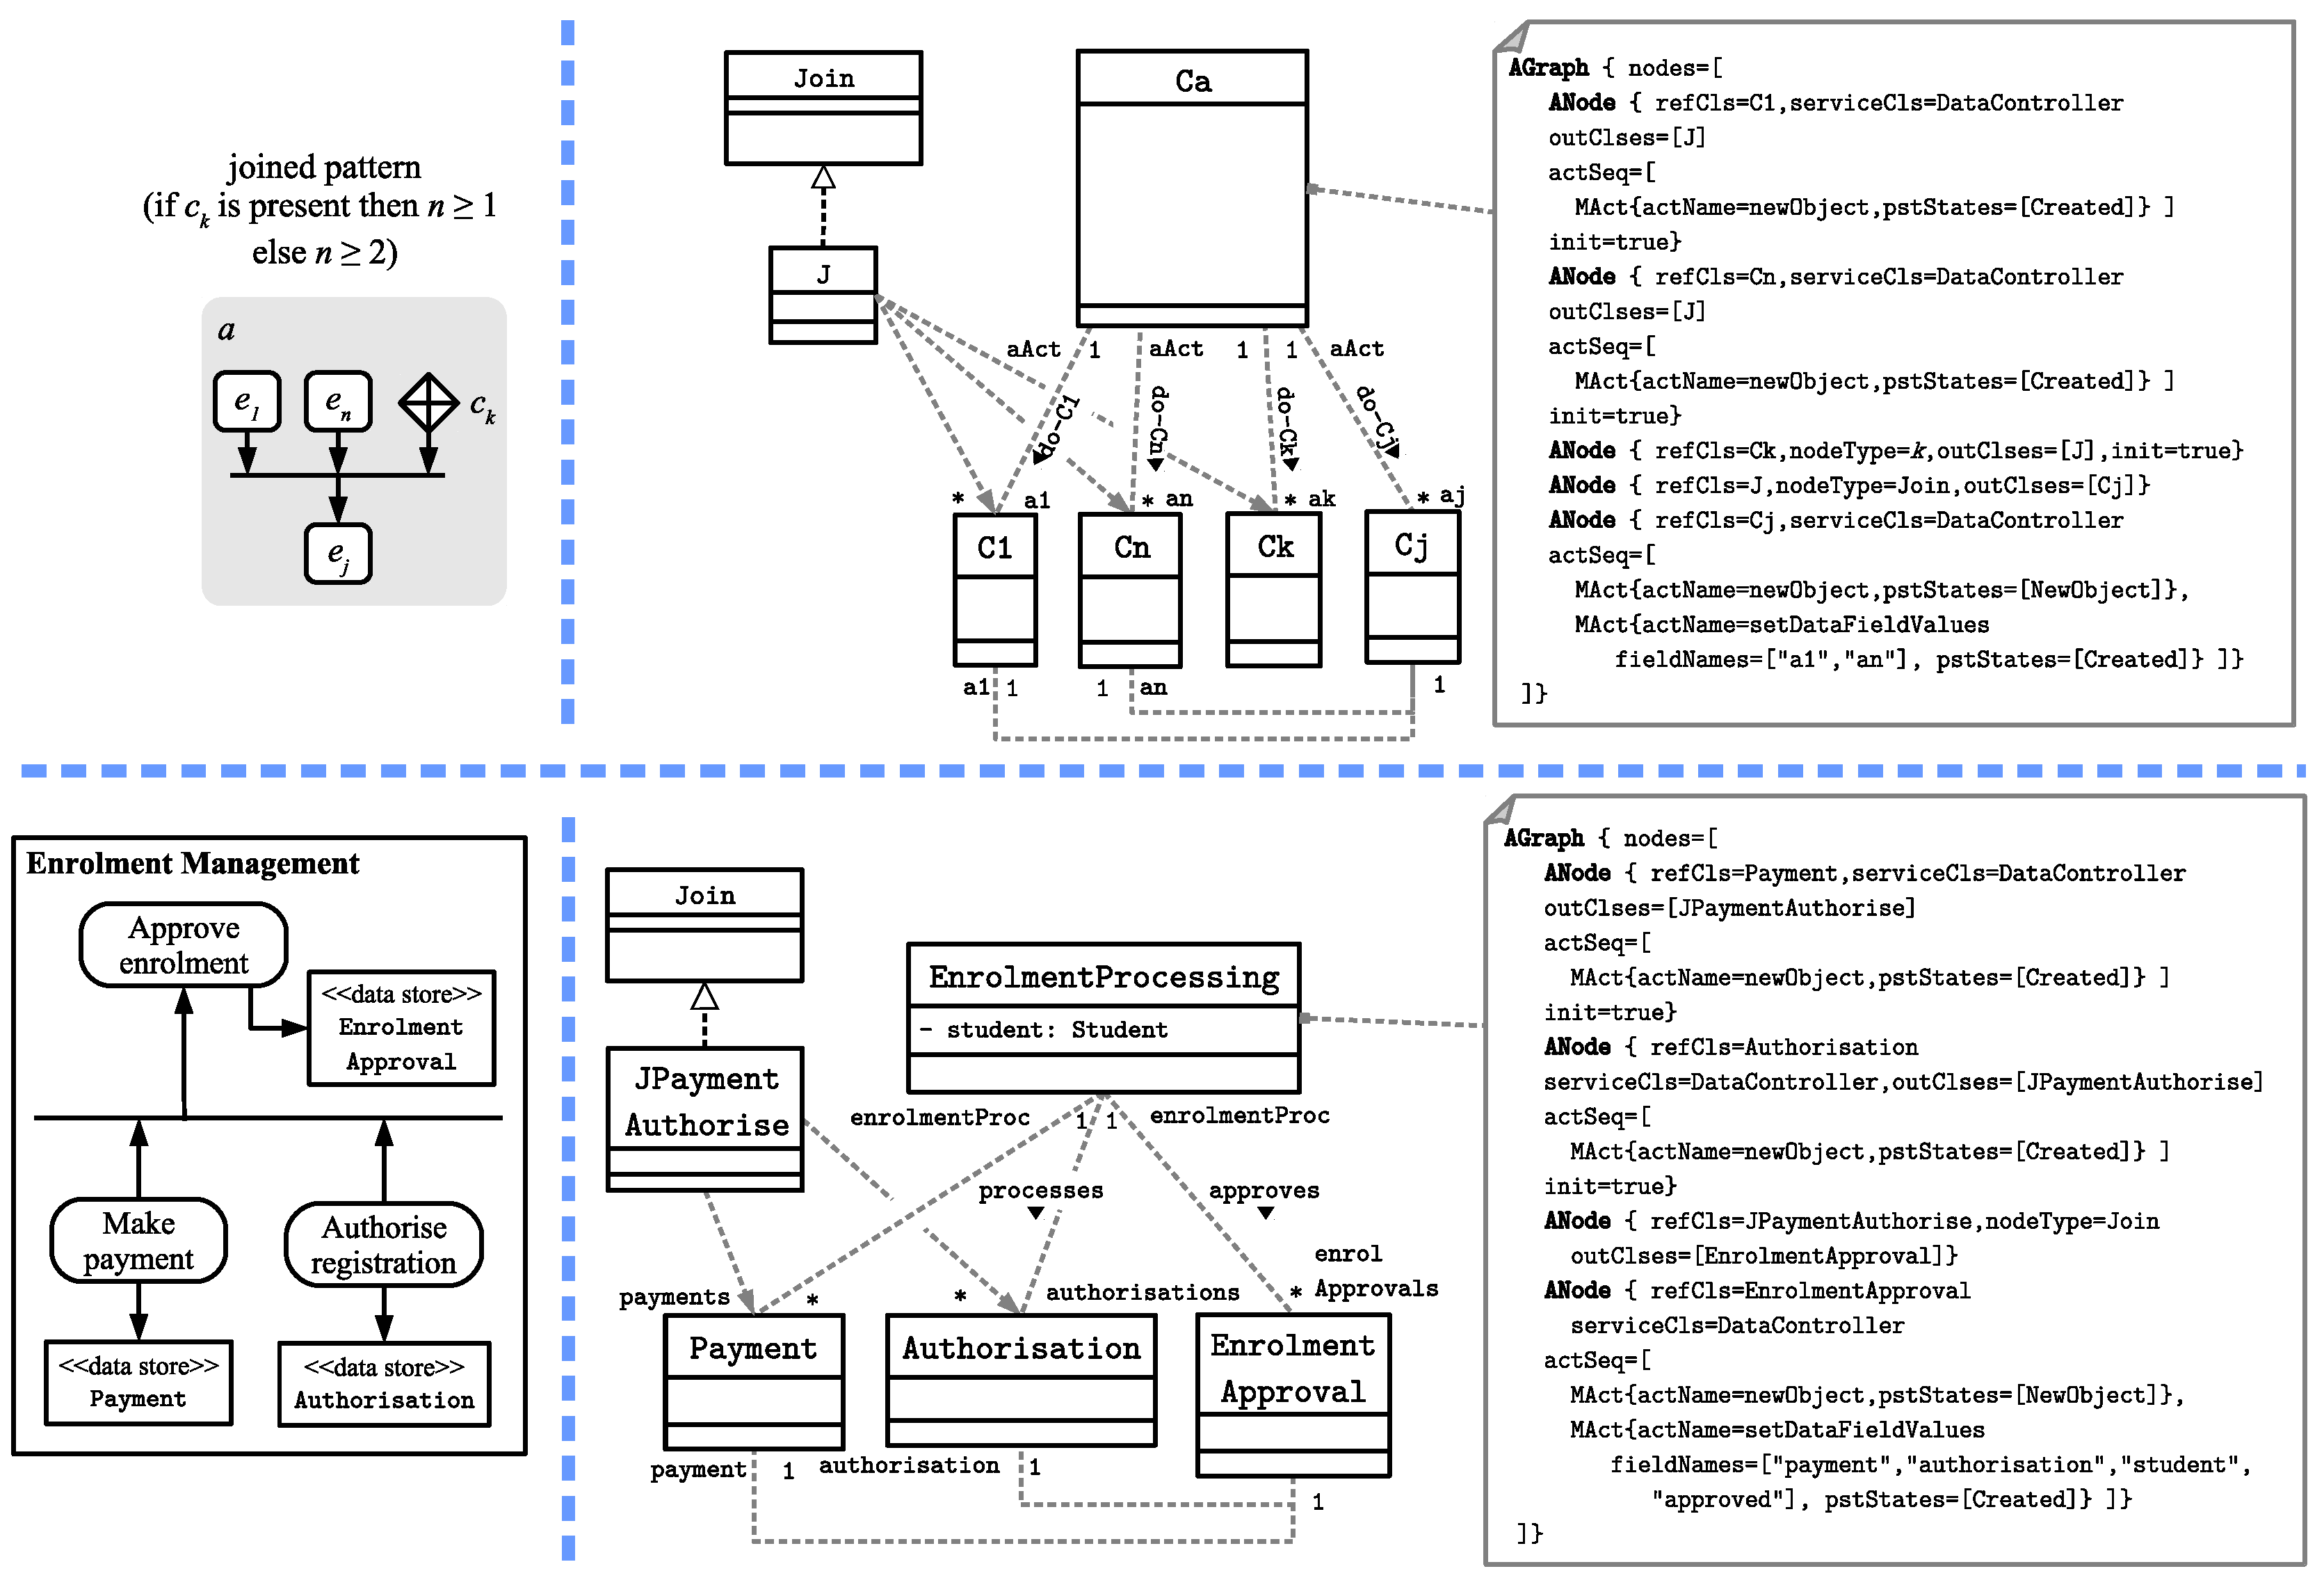
\includegraphics[scale=0.30 %0.3
  ]{case-study/joined-form}
\end{center}
\caption{The joined pattern form.} %
\label{fig:joined-form}
\end{figure*}
%
\begin{figure*}[ht]
\begin{center}
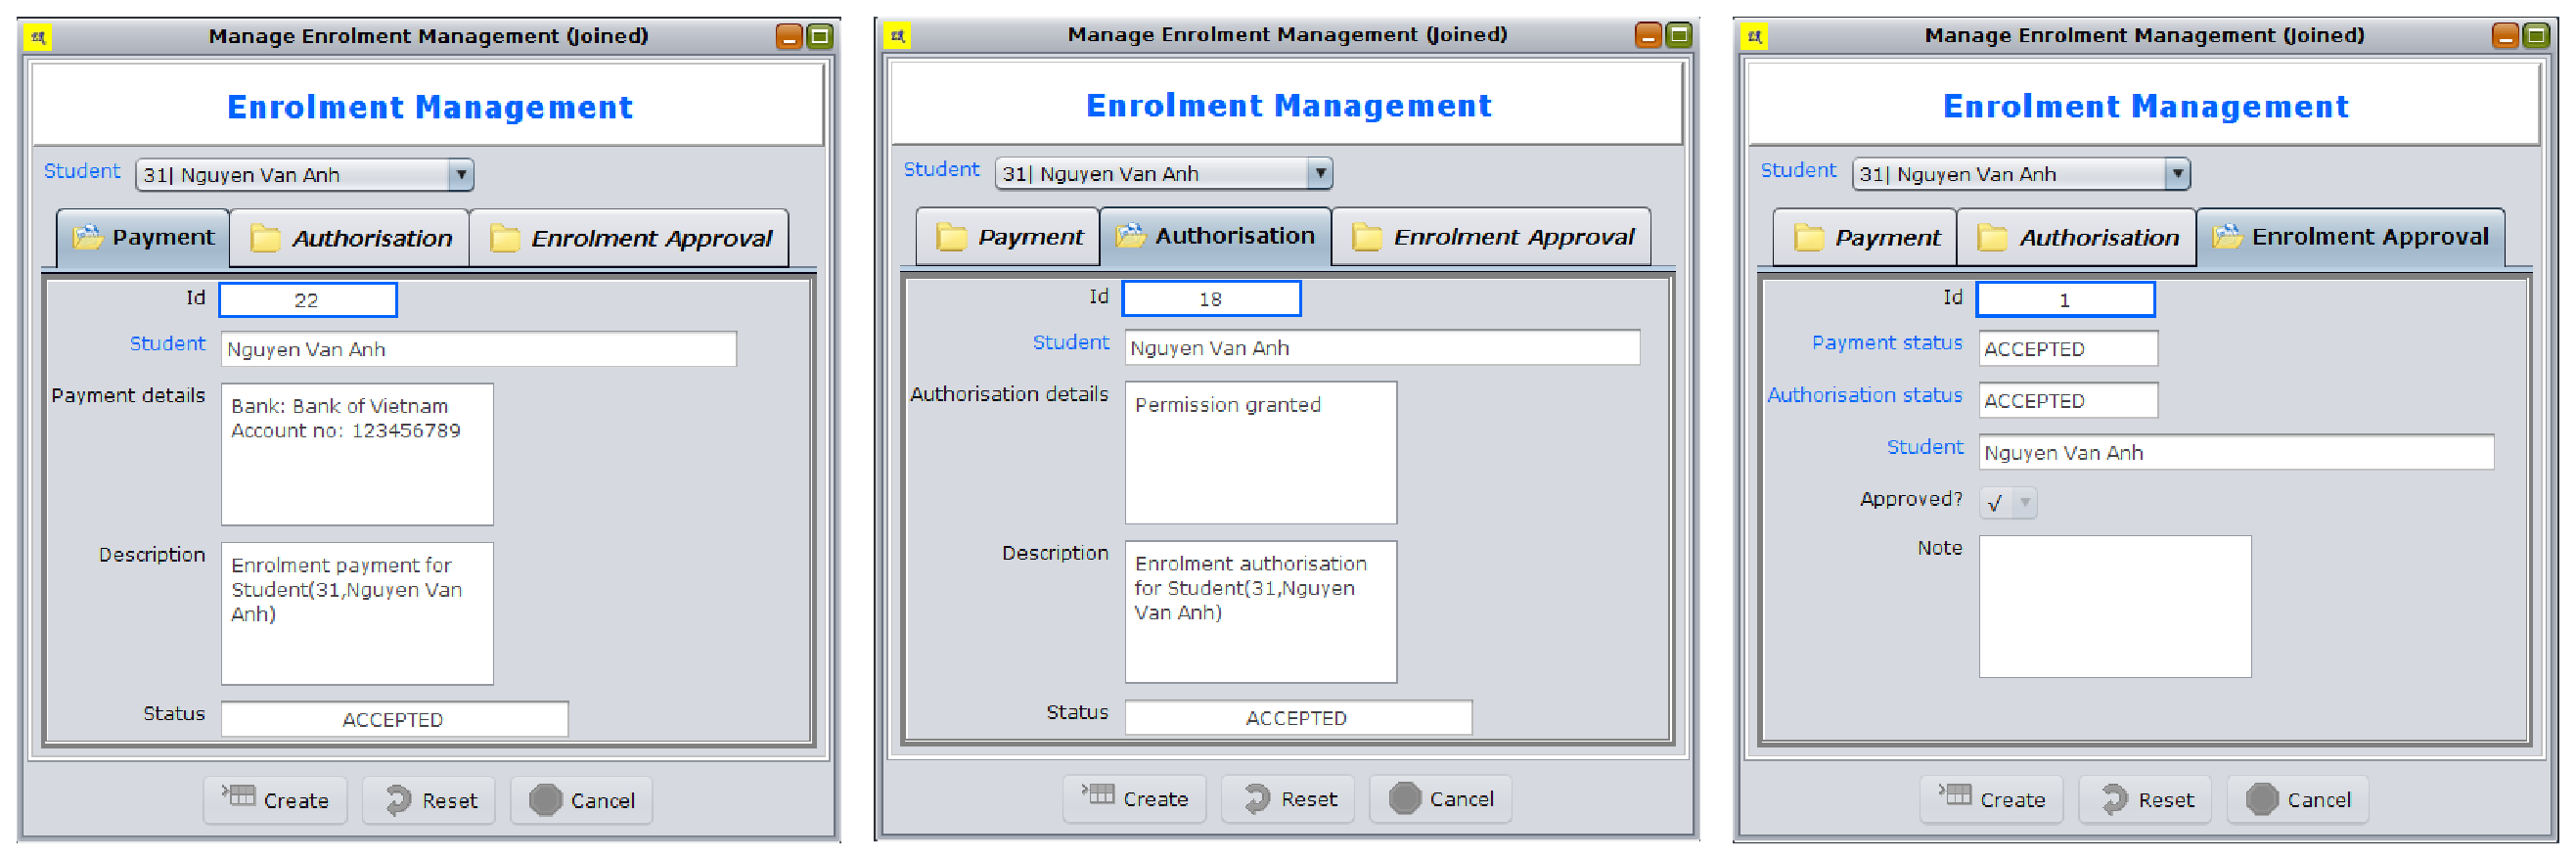
\includegraphics[scale=0.38 %0.4
  ]{case-study/joined-form-eg-gui}
\end{center}
\caption{The joined pattern form view of enrolment management activity.} %
\label{fig:joined-form-eg-gui}
\end{figure*}

The top-left of Figure~\ref{fig:joined-form} shows the UML activity model, while the top-right shows the template configured unified model. The activity class \clazz{Ca} has associations to the domain classes \clazz{C1}, \clazz{Cn}, \clazz{Ck}, and \clazz{Cj}. These classes are referenced by the activity nodes $ e_1 $, $ e_n $, $ c_k $, and $ e_j $ (\resp). Class \clazz{Cj} has two associations to \clazz{C1} and \clazz{Cn}, as it knows these two classes through object passing. Class \clazz{J} implements the interface \clazz{Join} for the join logic.

Similar to the decisional activity's template model, we create three (optional) weak dependency associations between class \clazz{J} and three domain classes \clazz{C1}, \clazz{Cn}, and \clazz{Ck}. In addition, we consider the case that the class \clazz{Ck} is not a decision class. When this class is a decision class, we unfold it into the template model.

The AGC consists of five \clazz{ANode}s. The first three \clazz{ANode}s configure the three start nodes $ e_1 $, $ e_n $, and $ c_k $; and thus they all have \attribn{init}=\code{true} and \attribn{outClses} pointing to the domain class \clazz{J}. This class, which realises the interface \clazz{Join}, is referenced by the fourth \clazz{ANode}. This \clazz{ANode} configures the join node, and thus has \attribn{nodeType}=\clazz{Join}. The last \clazz{ANode} configures the last node $ e_j $. It specifies two \clazz{MAct}, the second of which references the action  \membern{setDataFieldValues} which sets the view field values of the two fields \strq{a1} and \strq{an}. The input for this operation is the output of the operation \clazz{Join}.\membern{transf}.
%
\subsubsection*{Example}
The bottom of Figure~\ref{fig:joined-form} shows how the pattern is applied to another variant of the \courseman's enrolment management activity. The UML activity model of this variant involves joining two actions that concern the same \clazz{Student}, namely making payment ($e_1$) and registration authorisation ($e_2$), before concluding at the enrolment approval action. This last action decides, based on the results of the other two actions, whether or not to approve the student enrolment.

In this example: \clazz{Ca} = \clazz{EnrolmentMgmt}, $ n = 2 $, \clazz{C1} = \clazz{Payment}, \clazz{C2} = \clazz{Auhorisation}, \clazz{J} = \clazz{JPaymentAuthorise}, \clazz{Cj} = \clazz{EnrolmentApproval}.
Note that in addition to the newly added associations in the example model, class \clazz{EnrolmentProcessing} is added with a domain field \attribn{student}, which is used to obtain input from the user for a \clazz{Student}. This \clazz{Student} object is needed to initialise the payment and authorisation processes.

The three GUI snapshots of the example are shown in Figure~\ref{fig:joined-form-eg-gui}: the first snapshot is for making payment, the second is for registration authorisation, and the third is for enrolment approval.
%
\subsubsection{Merged Pattern Form} \label{sect:eval-expressiveness-merged}
%
\begin{figure*}[ht]
\begin{center}
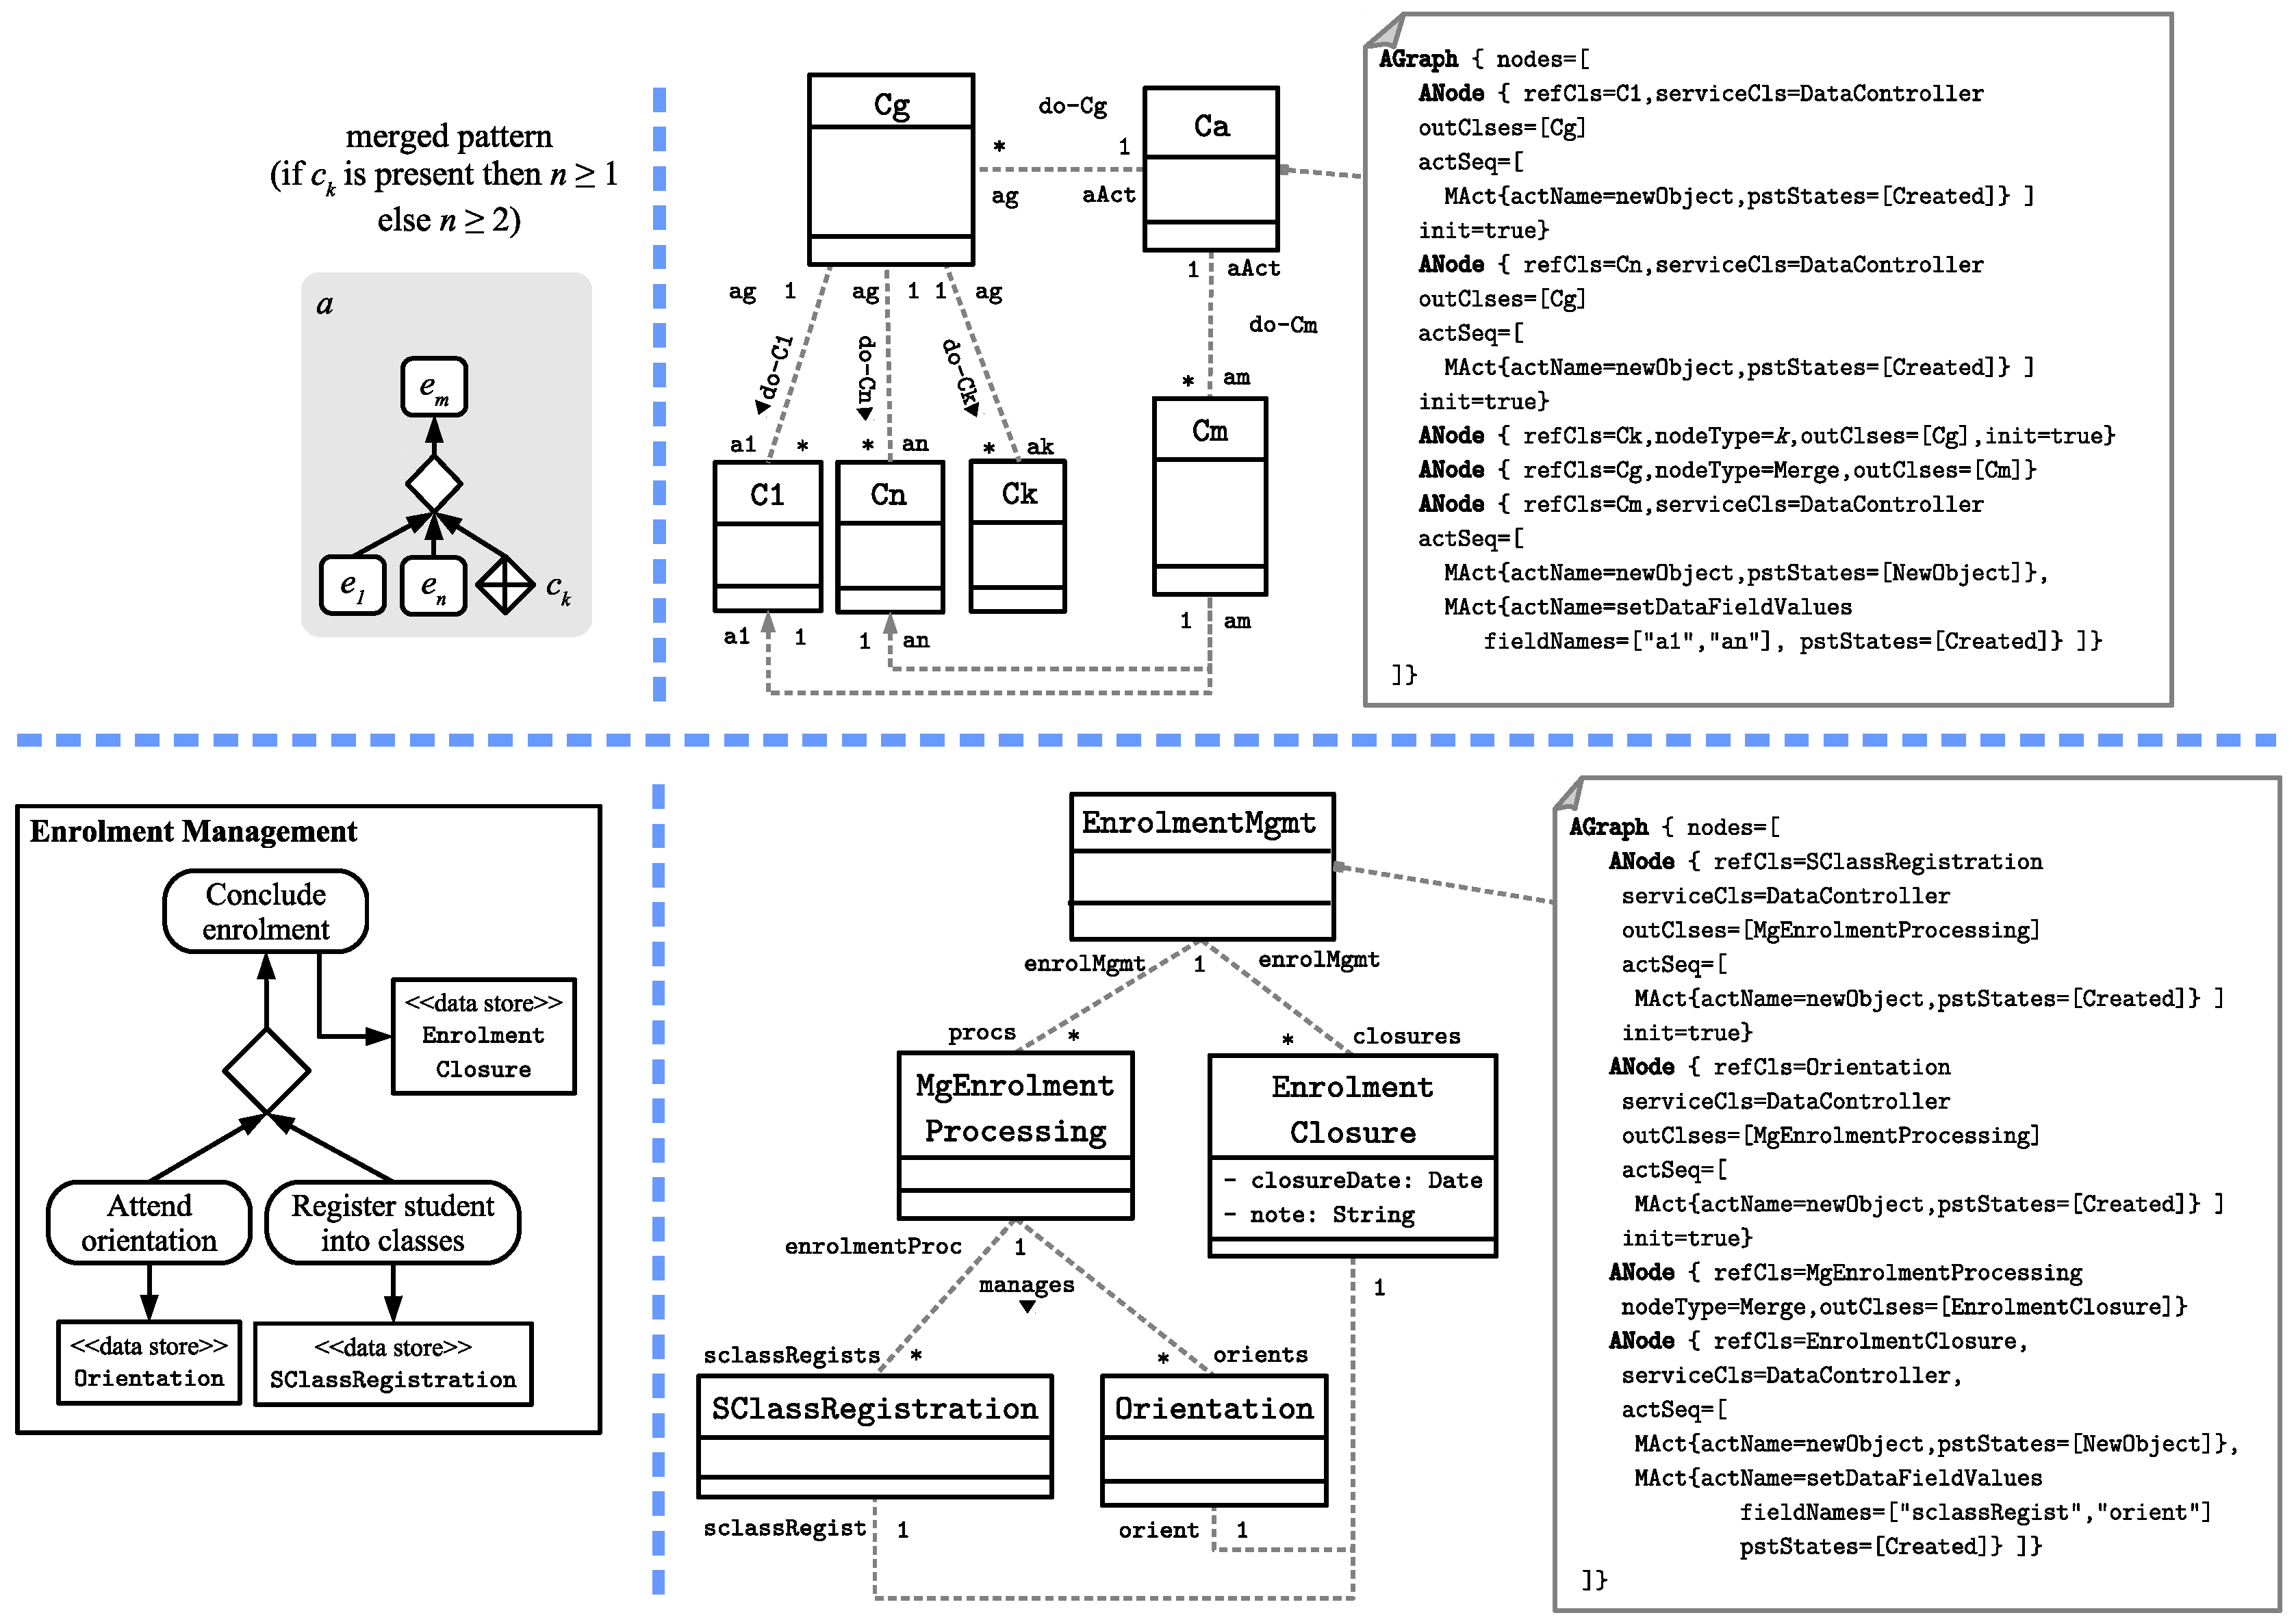
\includegraphics[scale=0.30 %0.3
  ]{case-study/merged-form}
\end{center}
\caption{The merged pattern form.} %
\label{fig:merged-form}
\end{figure*}
%
\begin{figure*}[ht]
\begin{center}
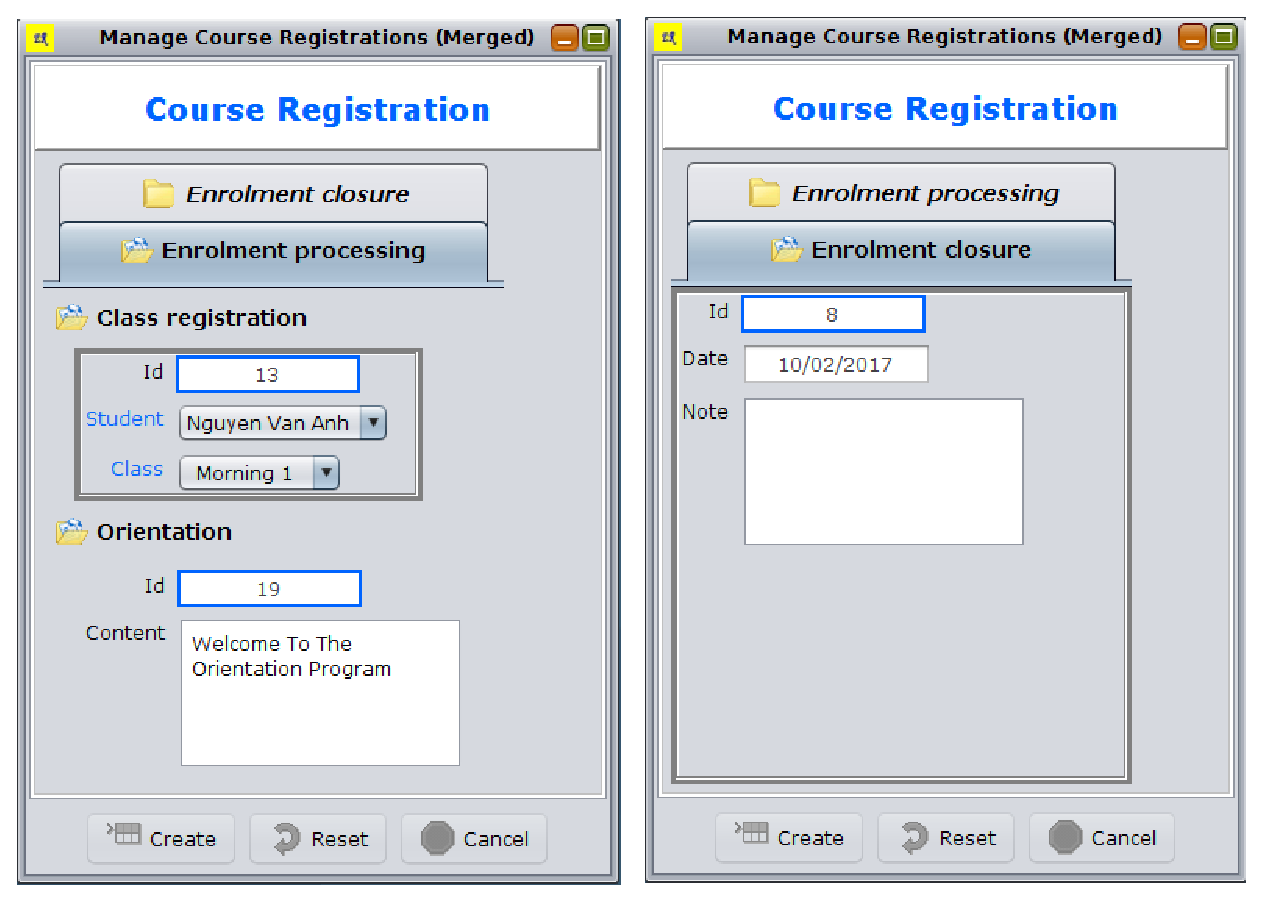
\includegraphics[scale=0.38 %0.4
  ]{case-study/merged-form-eg-gui}
\end{center}
\caption{The merged pattern form view of enrolment management activity.} %
\label{fig:merged-form-eg-gui}
\end{figure*}

The top-left of Figure~\ref{fig:merged-form} shows the UML activity model, while the top-right shows the template configured unified model. The activity class \clazz{Ca} has associations to the domain classes \clazz{Cg} and \clazz{Cm}. These classes are referenced by the merge node and the activity node $ e_m $ (\resp). Class \clazz{Cg} has associations to the domain classes of the other nodes, namely \clazz{C1}, \clazz{Cn}, and \clazz{Ck}. Class \clazz{Cm} has associations to class \clazz{C1} and \clazz{Cn} as it knows these two classes through object passing.

Similar to the decisional activity's template model, we consider the case that class \clazz{Ck} is not a decision class. When this class is a decision class, we unfold it into the template model.

The AGC is very similar to that of the join pattern form, except for the configuration of the fourth \clazz{ANode}, which specifies that the node type be \clazz{Merge} rather than \clazz{Join}.
%
\subsubsection*{Example}
The bottom of Figure~\ref{fig:merged-form} shows how the pattern is applied to another variant of the \courseman's enrolment management activity. The UML activity model of this variant involves merging two actions, namely student class registration ($e_1$) and attending an orientation ($e_2$), to conclude at the action enrolment closure ($e_m$). The assumption here is that students can perform any combination of the two actions $e_1, e_2$. The completion of any one action will lead to enrolment closure. The action that has not yet been performed can be performed by the students at some later time.

Action $e_2$ requires adding a new domain class named \clazz{Orientation} to the \Name{CourseMan}'s domain model. This class is displayed at the bottom right of Figure~\ref{fig:merged-form}. Thus, in this example: \clazz{Ca} = \clazz{EnrolmentMgmt}, $ n = 2 $, \clazz{C1} = \clazz{SClassRegistration}, \clazz{C2} = \clazz{Orientation}, \clazz{Cg} = \clazz{MgEnrolmentProcessing}, \clazz{Cm} = \clazz{EnrolmentClosure}. 

The GUI snapshots of the example are shown in Figure~\ref{fig:merged-form-eg-gui}. It shows a length-2 association chain from \clazz{EnrolmentMgmt} to \clazz{SClassRegistration} and \clazz{Orientation}. The first-level containment is that between the \clazz{EnrolmentMgmt}'s GUI and \clazz{MgEnrolmentProcessing}'s and \clazz{EnrolmentClosure}'s GUI. The second-level containment is that between \clazz{MgEnrolmentProcessing}'s GUI and \clazz{SClassRegistration}'s and \clazz{Orientation}'s GUI (the first and second snapshots). The \clazz{EnrolmentClosure}'s GUI is the third snapshot
%
\subsection{Required Coding Level} \label{sect:eval-rcl}
Required coding level (RCL) complements the expressiveness criterion in that it measures the extent to which a language allows ``...the properties of interest to be expressed without too much hard coding''~\cite{lamsweerde_formal_2000}.
Since \agl, to our knowledge, is the first aDSL of its type, we cannot compare \agl's RCL to other languages. Thus, we will measure the \agl's RCL using the ``compactness'' of the language's CSM (see Section~\ref{sect:agl-csm}). This is determined based on the reduction in the number of features in the $ASM$ through the transformation CM $\rightarrow$ CM$_T$. More precisely, \agl's RCL is the percentage of the number of CM$_T$'s features over the number of CM's. The smaller this percentage, the higher the reduction in the number of features in the CSM and, thus, the more compact the CSM.

It is clear from Figures~\ref{fig:agl-cm} and~\ref{fig:agl-cmt} that \agl's RCL $ = \frac{3}{9}$ or approximately 33\%. Specifically, Figure~\ref{fig:agl-cm} shows that the number of meta-concepts of the CM involved in the transformation is 9. These exclude the four meta-concepts (\clazz{ActName}, \clazz{State}, \clazz{Decision} and \clazz{Join}) that are transferred directly to CM$_T$. On the other hand, Figure~\ref{fig:agl-cmt} shows that 3 meta-concepts result from the transformation (including \clazz{AGraph}, \clazz{ANode} and \clazz{MAct}). Therefore, \agl~can have a CSM that significantly reduces the number of meta-concepts required to write an AGC to only about one third. 
%
\subsection{Constructibility} \label{sect:eval-construct}
This is the extent to which a language provides ``...facilities for building complex specifications in a piecewise, incremental way''\cite{lamsweerde_formal_2000}. For \agl, the language's embedment in the host OOPL allows it to take for granted the general construction capabilities of the host language platform and those provided by modern IDEs (\eg Eclipse). More specifically, using an IDE a developer can syntactically and statically check an AGC at compile time. In addition, she can easily import and reference a domain class in an AGC and have this AGC automatically updated (through refactoring) when the domain class is renamed or relocated.

More importantly, the AGC can be constructed incrementally with the domain model. This is due to a property of our activity graph model (discussed in Section~\ref{sect:agl-conceptual-model}) that the nodes and edges of an activity graph are mapped to the domain classes and their associations.

Further, we would develop automated techniques to ease the construction of AGC. Intuitively, for example, a technique would be to generate a default AGC for an activity and to allow the developer to customise it. We plan to investigate techniques such as this as part of future work.